%%%%%%%%%%%%%%%%%%%%%%%%%%%%%%%%%%%%%%%%%%%%%%%%%%%%%%%%%%%%%%%%%%%%%%%%
% Plantilla TFG/TFM
% Escuela Politécnica Superior de la Universidad de Alicante
% Realizado por: Jose Manuel Requena Plens
% Contacto: info@jmrplens.com / Telegram:@jmrplens
%%%%%%%%%%%%%%%%%%%%%%%%%%%%%%%%%%%%%%%%%%%%%%%%%%%%%%%%%%%%%%%%%%%%%%%%

\chapter{Trabajo Futuro}

El sistema desarrollado ha servido como base conceptual y técnica para la aplicación de soluciones similares en un entorno profesional real. En particular, los conocimientos adquiridos durante el diseño e implementación desl sistema de monitorización de red han sido aplicados posteriormente en el desarrollo de una herramienta destinada a la gestión de switches en el Hospital Universitario Virgen de la Arrixaca, en Murcia.

En este contexto profesional, se ha desarrollado una aplicación web orientada a la supervisión y gestión de la infraestructura de red del hospital, con especial énfasis en el control del uso de VLANs y en la gestión de los puertos de los switches. Uno de los principales objetivos de esta herramienta es identifica puertos que no rpesentan conectividad durante un periodo prolongado de tiempo, dado que, según las políticas internas del centro, los puertos que permanecen inactivos durante más de seis meses deben ser liberados para optimizar el uso de recursos de red.

La aplicación desarrollada permite visualizar de forma centralizada el estado de los puertos de los switches, diferenciando entre puertos activos y puertos libres, así como el uso de las distintas VLANs configuradas en la red. Esta funcionalidad resulta especialmente relevante en un entorno hospitalario, donde la gestión eficiente y ordenada de la red es crítica para garantizar la disponibilidad de los servicios y la correcta conexión de los sistemas clínicos.

En la Figura~\ref{fig:trabajo-real-dashboard} se muestra una vista general de la herramienta desarrollada, donde se aprecia la presentación visual de la información y el enfoque orientado a la supervisión rápida del estado de la red.

\begin{figure}[H]
  \centering
  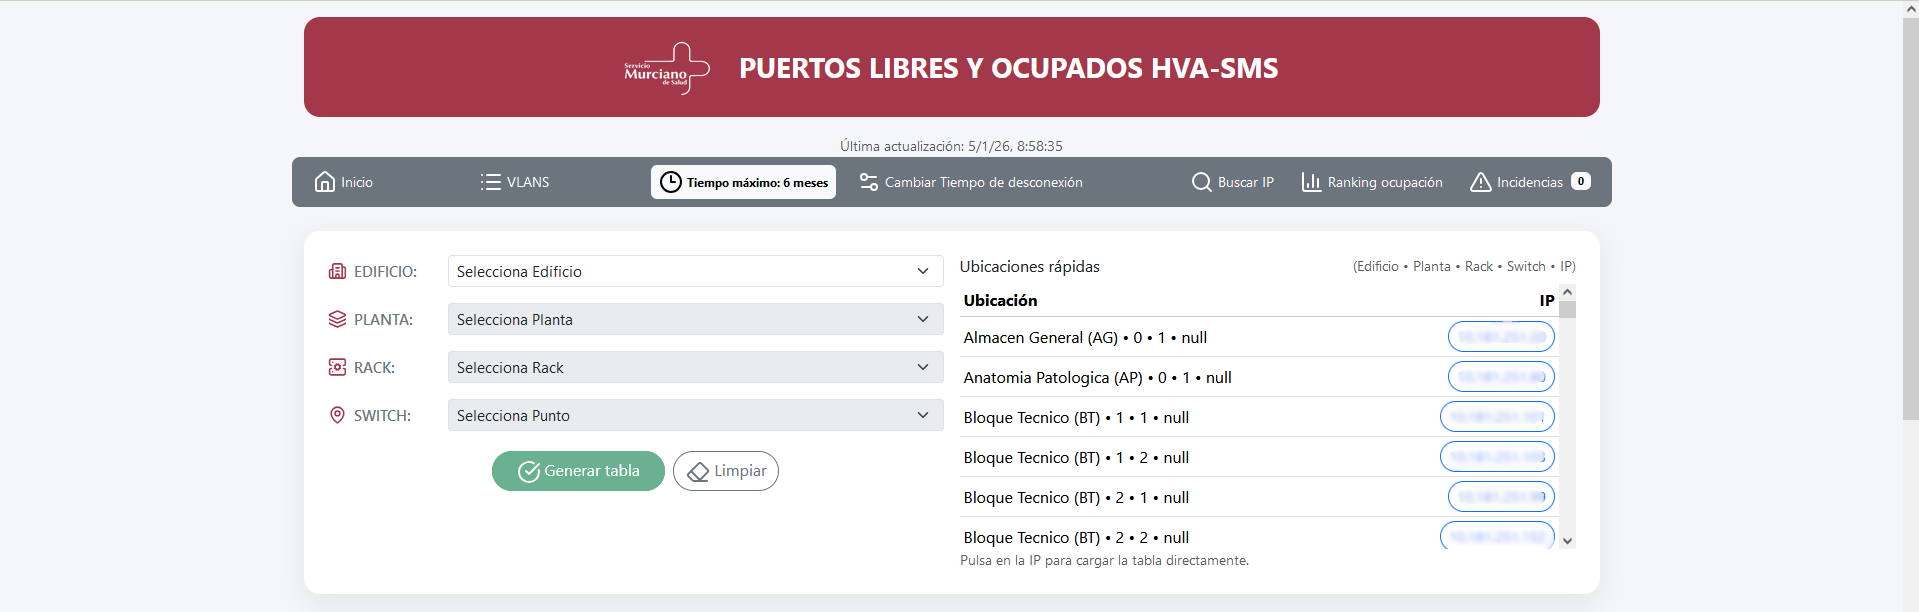
\includegraphics[width=\textwidth]{imagenes/PRIMERA_CAPTURA - Editada.png}
  \caption{Vista general de la aplicación web desarrollada para la gestión de switches en el entorno hospitalario.}
  \label{fig:trabajo-real-dashboard}
\end{figure}

La gestión específica de VLANs constituye otro de los elementos clave de esta aplicación. A través de la interfaz web, es posible conocer las VLANs en uso y su distribución, facilitando tareas de administración y planificación de la red. 

Asimismo, la aplicación incorpora funcionalidades específicas para la identificación y la gestión de puertos sin conexión, permitiendo detectar de forma automática aquellos puertos que no han registrado actividad durante un perido prolongado. Esta información facilita la toma de decisiones relacionadas con la liberación y reutilización de recursos de red. En la Figura~\ref{fig:trabajo-real-vlans} y la Figura~\ref{fig:trabajo-real-puertos} se muestran ejemplos de esta funcionalidad.

\begin{figure}[H]
  \centering
  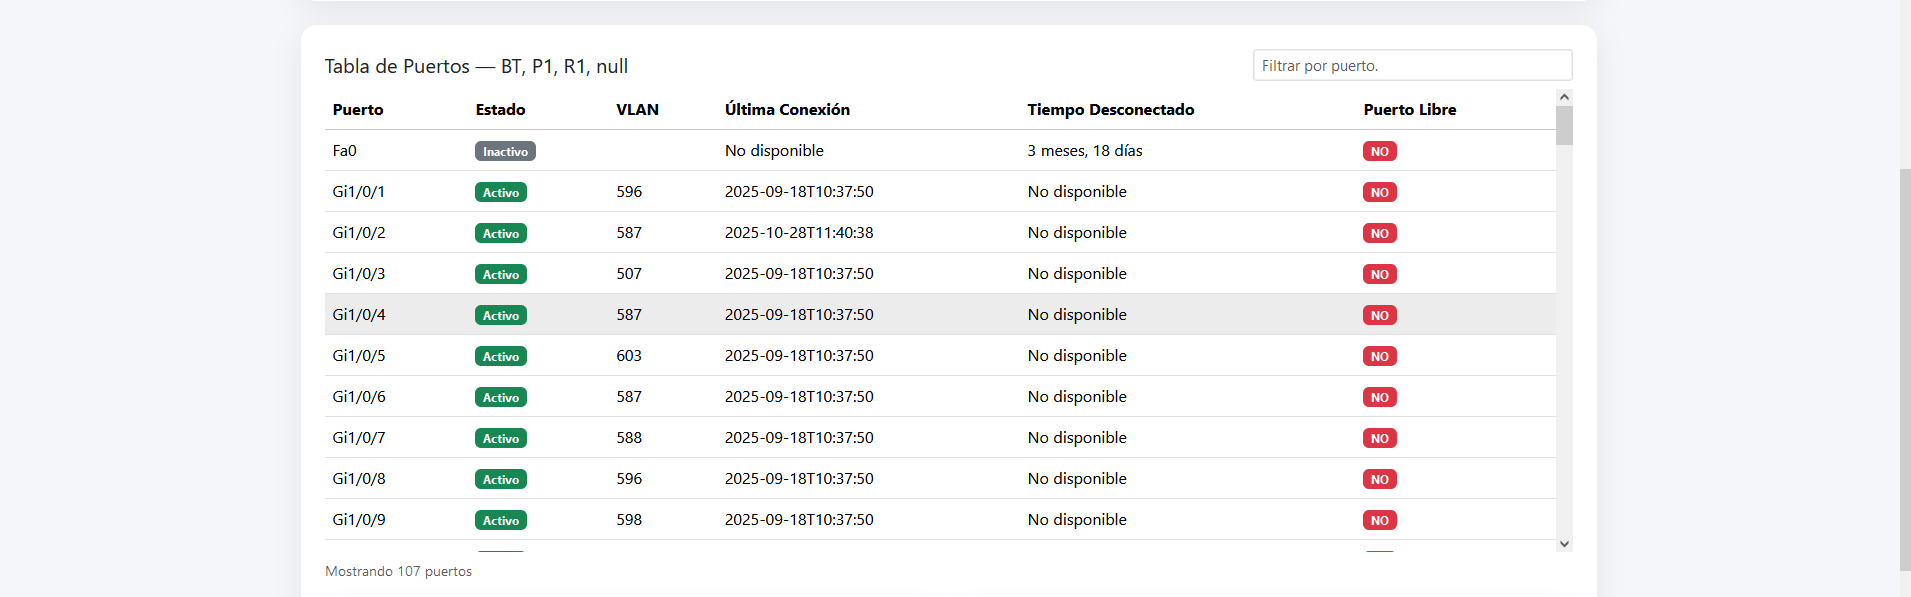
\includegraphics[width=\textwidth]{imagenes/SEGUNDA_CAPTURA.png}
  \caption{Gestión y supervisión de puertos libres y ocupados en switches del entorno hospitalario.}
  \label{fig:trabajo-real-vlans}
\end{figure}

\begin{figure}[H]
  \centering
  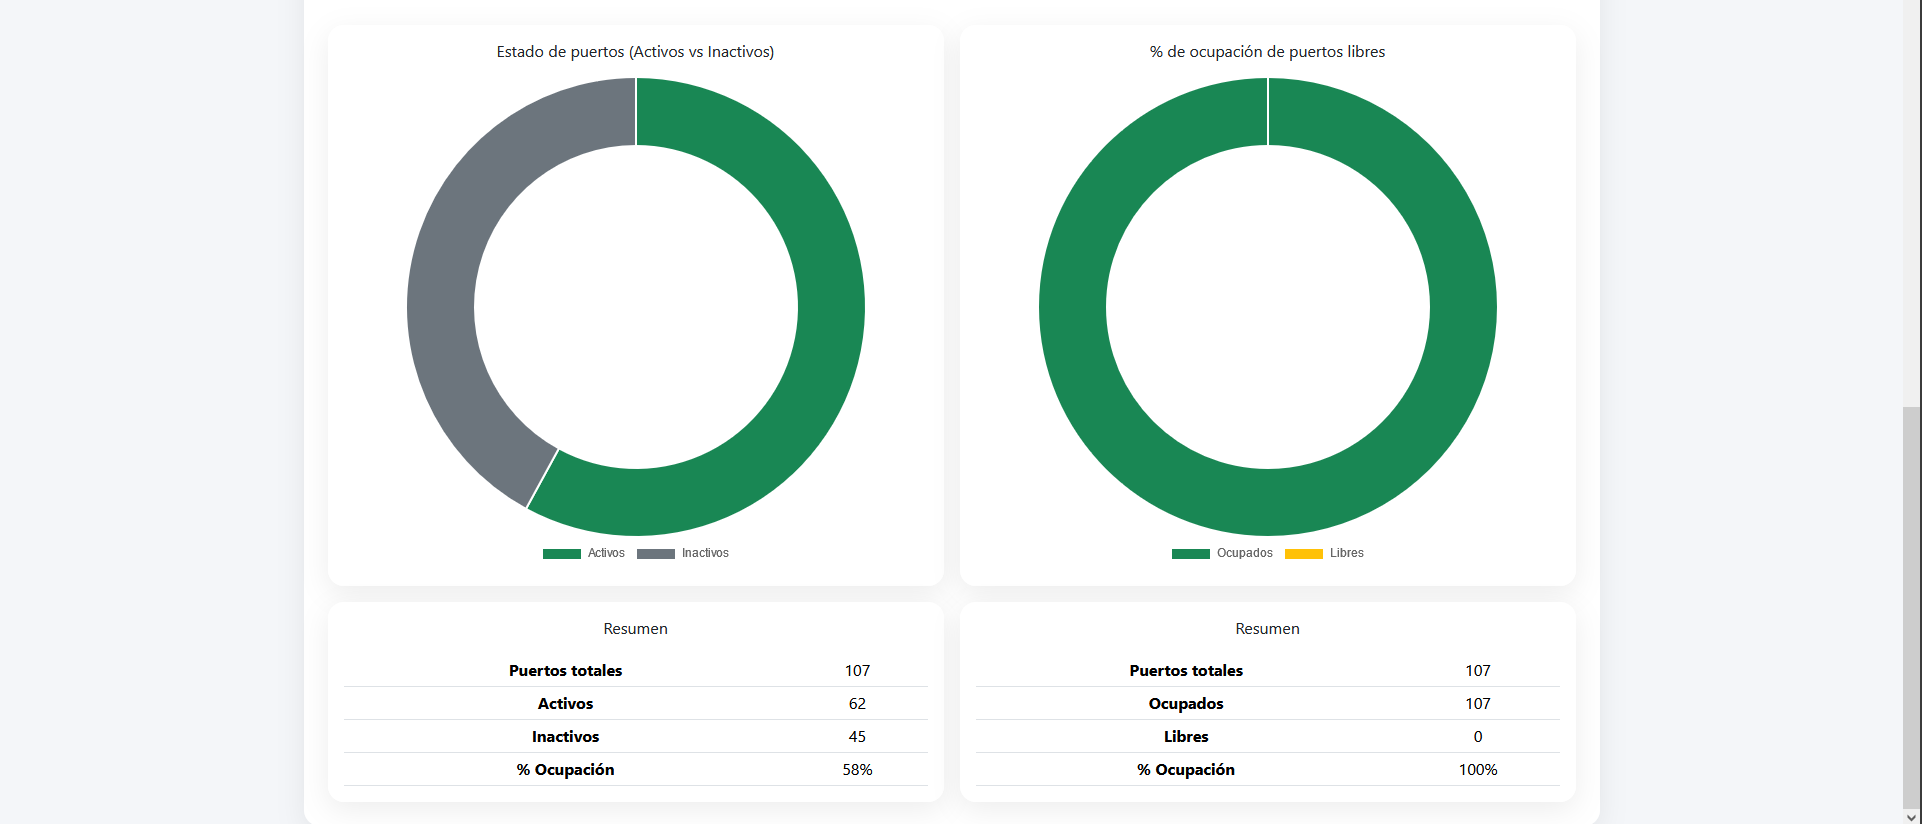
\includegraphics[width=\textwidth]{imagenes/TERCERA_CAPTURA.png}
  \caption{Gestión y supervisión de puertos libres y ocupados de manera gráfica.}
  \label{fig:trabajo-real-puertos}
\end{figure}

La experencia adquirida durante la realización del Trabajo Final de Máster ha sido fundamental para abordar el desarrollo de esta solución en un entorno real, permitiendo aplicar conceptos relacionados con la monitorización de red, la automatización de tareas y la visualización de información de forma estructurada. En este sentido, el proyecto desarrollado en el ámbito académico ha constituido un punto de partida clave para la evolución hacia soluciones aplicadas directamente en el entorno profesional, reforzando la utilidad práctica de los conocimientos adquiridos durante el máster.


